\chapter{playback engine}
\renewcommand{\baselinestretch}{\mystretch}
\label{chap:Playback}
%\setlength{\parindent}{0pt}

Based on the exported data format, an independent playback engine was developed and integrated into Vixen. \wn{6}

\cmt{The details of implementation, processing, performance critical steps skipped. \wn{6}}

\cmt{XML reading, serialiser}

\cmt{User interface..., does not support preview}

\cmt{Insert screenshots...}

\section{Performance and optimisations}

\cmt{Export performance and file sizes}

\cmt{Threading and mutex lock structure difference}

\cmt{Dictionary lookup replaced \wn{14}}

\fref{fig:playback} shows the performance of the playback engine. At the first and the last few seconds, the playback stopped, the system was using the original execution engine in idle. However, this engine still uses about $30 \%$ of CPU time. But, as soon as playback started, CPU usages drops to around $6 \%$ with stable refresh frame rates.

\begin{figure}[t]
    \centering
    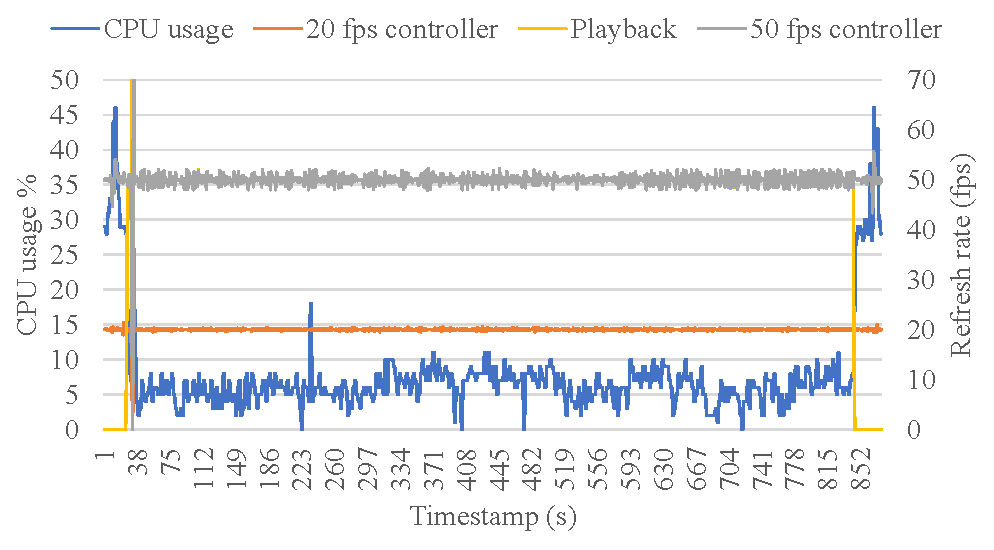
\includegraphics[width=0.8\columnwidth]{playback}
    \caption{Performance of new playback engine}
    \label{fig:playback}
\end{figure}

\section{Integration}

A separate menu entry was added to control the new playback engine. When the engine starts, it takes priority over the original execution engine.

\section{Audio playback}

The network configuration XML file generated from export was modified to include the audio media file used in the original sequence. This field was later used in the playback engine for audio playback, using the same audio functions from sequence playback. \wn{7}

\section{Scheduler integration}

The playback control was also integrated with built-in schedulers. It can therefore be scheduled to execute multiple times at specific time, possibly with original sequence schedules. \wn{8}

\cmt{Insert screenshots...}

The scheduler pre-process all scheduled items first. The sequences need to be pre-rendered, which can take a significant amount of time. The new playback engine does not need pre-process, can be directly executed within seconds.
